

% movido a implementación - iteración 2
\subsubsection{Geolocalizar los Lugares}
\label{sub:fronted_lugares}

El hecho de localizar un lugar. significa que se lo va a ubicar sobre un mapa gracias a sus coordenadas, tales que se encuentran almacenadas en la base de datos. por lo tanto es necesario hacer una petición al \emph{endpoint} del REST API dedicado a obtener de la base de datos la información de un lugar, la cual se muestra a continuación. \\

\begin{center}
  \begin{verbatim}
    router.get('/:id', places.getPlace);
  \end{verbatim}
\end{center}

El método asociado, ver codigo \ref{getPlace}, obtiene las coordenadas en formato GeoJSON, el cual es formato estándar al trabajar con información geográfica en plataformas que usan JavaScript, que es el caso del navegador. \\

\begin{center}
 \begin{lstlisting}[label=getPlace,caption=Método para obtener la información de un lugar.]

   var getPlace = (req, res) => {
     var id = req.params.id;
     var raw = `SELECT
            ST_AsGeoJSON(p.geom)::json As geometry,
            p.name,
            p.description,
            p.phone,
            p.level,
            p.gid As id,
            (string_agg(i.cloudinary_public_id, ',')) as images
            FROM place p
            LEFT JOIN place_images i ON p.gid = i.place_id
            WHERE p.gid = ${id}
            GROUP BY p.gid;`;

     Bookshelf.knex.raw(raw)
       .then((data) => {
         res.json(data.rows[0]);
       })
       .catch((error) => {
         console.log(error);
         res.send("Error");
       });
   };

 \end{lstlisting}
\end{center}


Entonces solo faltaría ubicar el lugar utilizando sus coordenadas sobre un mapa, para resolver esta tarea se utilizó \emph{ember-leaflet}, una librería creada para manipular mapas y diseñada especialmente  para su implementación en dispositivos móviles.\\

Para instalar esta librería solo se necesita ejecutar el siguiente comando y posteriormente ya se puede empezar a utilizarla.\\

\begin{verbatim}
$ ember install ember-leaflet
\end{verbatim}


% Primeramente es necesario conocer las coordenadas del ``lugar'', para lo cual se hará un \emph{request} al API de la aplicación para obtener la información del ``lugar'', el URI designado para esta tarea es \verb|places/:id| usando el verbo HTTP \emph{GET}, para mejorar el manejo de la coordenadas se utilizó el formato \emph{GeoJSON},
En \emph{EmberJS} las coordenadas son procesadas dentro del \emph{controlador}, el cual maneja las variables implementadas en el \emph{template}, tal como se puede observar en el siguiente codigo \ref{leafletMap}, las variables: \emph{lat} y \emph{lng} llamadas dentro del tag \verb|#leaflet-map|, que son la latitud y longitud respectivamente del punto georeferenciado. \\

% \begin{center}
%   \begin{verbatim}
%     var maker = new google.maps.Marker({
%       position: new google.maps.LatLng( lat, lng  )
%       map: UMSS.map
%     });
%   \end{verbatim}
% \end{center}

\begin{center}
 \begin{lstlisting}[label=leafletMap,caption=Método para obtener la información de un lugar.]

   {{#leaflet-map lat=lat lng=lng zoom=zoom}}
     {{tile-layer url="http://{s}.tile.openstreetmap.fr/hot/{z}/{x}/{y}.png" }}
       {{#marker-layer location=location}}
         <h3>{{model.name}}</h3>
         {{model.description}} <br>
         <strong>telf:</strong> {{model.phone}} <br>
         <strong>piso </strong>#{{model.level}}
     {{/marker-layer}}
   {{/leaflet-map}}

 \end{lstlisting}
\end{center}

\emph{Ember-leaflet} permite manejar distintos servidores de mapas, pero se escogió \emph{Open Street Maps} por su facilidad de uso, ser \emph{open source} y al no necesitar adquirir licencias para su uso, el resultado del anterior codigo se puede apreciar en la figura \ref{fig:ember_leaflet}. \\

\begin{figure}[H]
     \begin{center}
       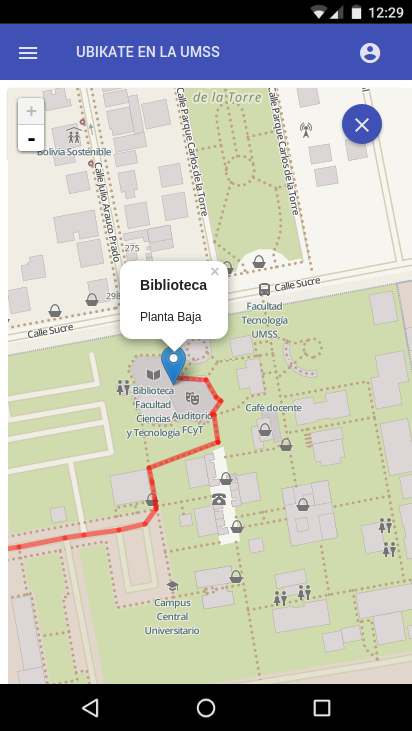
\includegraphics[width=0.3\textwidth]{ember_leaflet}

       \caption{ Mapa mostrado con la ayuda de \emph{ember-leaflet}}
       \label{fig:ember_leaflet}
       \caption*{Fuente: Elaboración propia.}
     \end{center}
\end{figure}


\emph{Ember-leaflet} también permite personalizar los elementos del mapa que se estan renderizando, por ejemplo como parte de las tareas de esta iteración, es necesario añadir un \emph{marcador} sobre el lugar en el mapa y  \emph{ember-leaflet} permite hacer tal cosa, así como también personalizar el marcador e incluir la información del lugar, como se puede ver en el codigo \ref{leafletMap}, dentro del \emph{tag} \verb|#marker-layer| se está dando formato a la información del lugar, el resultado de esta tarea se puede apreciar en la figura \ref{fig:baquita_place}. \\


\begin{figure}[H]
 \begin{center}
   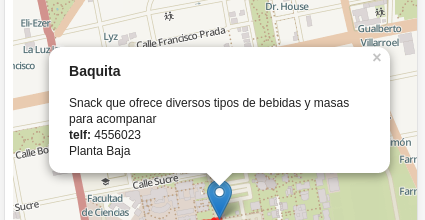
\includegraphics[width=0.8\textwidth]{iteration2/baquita_place}
   \caption{Marcador con la información de un lugar.}
   \label{fig:baquita_place}
   \caption*{Fuente: Elaboración propia.}
 \end{center}
\end{figure}


% Para poder acceder a la anterior vista, es necesario en primer lugar seleccionarlo de una lista





% \begin{figure}[H]
%  \begin{center}
%    \caption{Vista de la lista de Lugares registrados en el sistema.}
%    \label{fig:places_index}
%    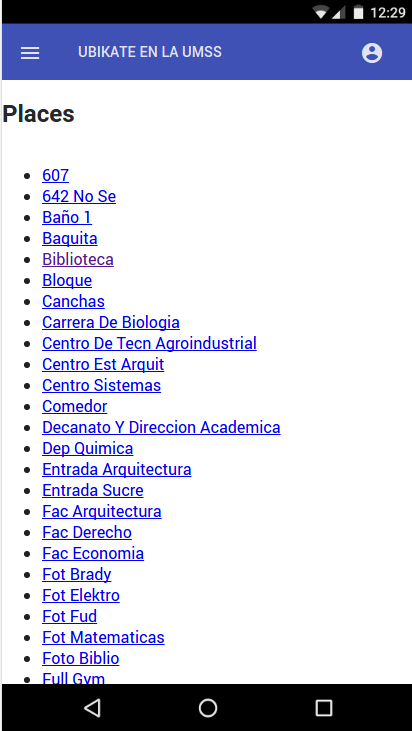
\includegraphics[width=0.5\textwidth]{iteration1/places_index}
%    \caption*{Fuente: Elaboración propia}
%  \end{center}
% \end{figure}


% \begin{figure}[H]
%  \begin{center}
%    \caption{Vista de la búsqueda de lugares a través de un cajón de búsqueda.}
%    \label{fig:places_search}
%    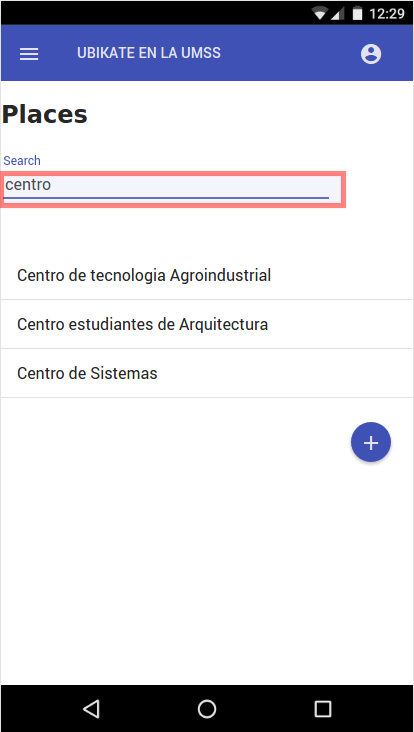
\includegraphics[width=0.5\textwidth]{iteration1/places_search}
%    \caption*{Fuente: Elaboración propia}
%  \end{center}
% \end{figure}


% Para implementar esta funcionalidad del sistema fue necesario utilizar las funcionalidad de Ember JS.
%
% \begin{verbatim}
%  {{#paper-item class="md-1-line" onClick=(transition-to 'places.show' place)}}
%      <div class="md-list-item-text">
%          <span>{{place.name}}</span>
%      </div>
%  {{/paper-item}}
% \end{verbatim}
%
%
% \begin{figure}[H]
%    \label{fig:place_show}
%    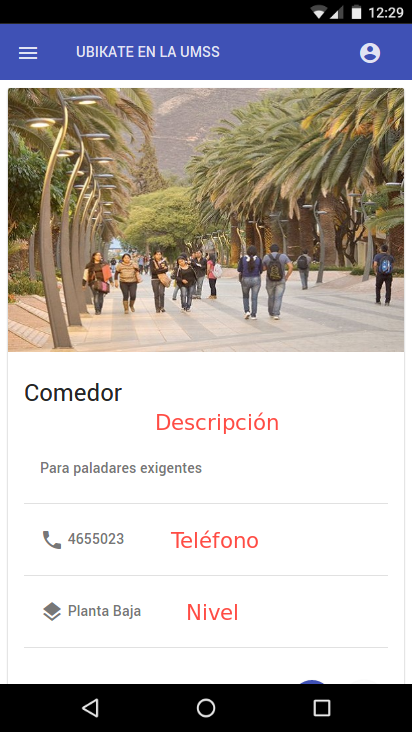
\includegraphics[width=0.5\textwidth]{iteration1/place_show}
%    \caption*{Fuente: Elaboración propia}
%  \end{center}
% \end{figure}

% movido a implementacion - iteracion 2


\subsubsection{Geolocalizar los Usuarios}
\label{sub:Manejo de Usuarios}

Para encontrar la ruta más corta entre el usuario y un lugar hay que conocer la locación del usuario, el punto geolocalizado de la ubicación del usuario se lo obtuvo usando el API de geolocalización propio de HTML5. \\

La especificación de HTML5 indica que el navegador puede acceder y usar los recursos nativos de un \emph{smartphone}, la locación del usuario es encontrada mediante la triangulación de Coordenadas por GPS (el mas exacto a la hora de encontrar la locación del dispositivo), Wi-Fi, GSM o CDMA. \\

En el navegador solo es necesaria la ejecución de la siguiente línea para poder obtener la posición actual del usuario usando el API de geolocalización de HTML5.

% Si se quiere saber la ruta más corta entre el usuario y un lugar, es necesario conocer la locación del usuario y hay que tomar en cuenta que esta información no se encuentra en la base de datos. Por lo tanto es necesario obtener el punto georreferenciado del usuario como punto de inicio de la ruta más corta, para lo cual se utilizó el API de geolocalización propio de HTML5, la especificación de HTML5 indica que el navegador puede acceder y usar los recursos nativos de un smartphone pero es necesaria la aceptación del usuario mediante un mensaje que el navegador despliega, la locación es encontrada mediante la triangulación de Coordenadas por GPS (el mas exacto a la hora de encontrar la locación del dispositivo), Wi-Fi, GSM o CDMA. Solo es necesaria la ejecución de la siguiente línea para poder obtener la posición actual del usuario usando el API de geolocalización de HTML5. \\

\begin{verbatim}
 var coords = Geolocation.getCurrentPosition();
 var latitud = coords.latitude;
 var longitud = coords.longitude;
\end{verbatim}

Donde la \emph{latitud} y \emph{longitud} obtenidas son fácilmente trasladadas al mapa usando \emph{ember-leaflet} y mediante un marcador se puede visualizar la ubicación actual del usuario, como se puede ver en la siguiente figura \ref{fig:location_marker}.

\begin{figure}[H]
 \begin{center}
   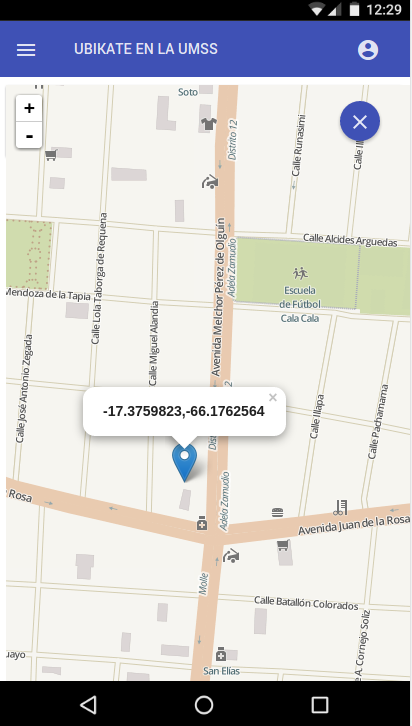
\includegraphics[width=0.3\textwidth]{iteration2/location_marker}
   \caption{Marcador sobre la posición actual del usuario.}
   \label{fig:location_marker}
   \caption*{Fuente: Elaboración propia.}
 \end{center}
\end{figure}


% \subsubsection{Manejo de Usuarios}
% \label{sub:Manejo de Usuarios}
%
% Si se quiere saber la ruta más corta entre el usuario y un lugar conocer la locación del usuario, hay que tomar en cuenta que esta información no se encuentra en la base de datos, es necesario obtener el punto georreferenciado del usuario como punto de inicio, para lo cual se utilizó el API de geolocalización propio de HTML5, la especificación de HTML5 indica que el navegador puede acceder y usar los recursos nativos de un smartphone pero es necesaria la aceptación del usuario mediante un mensaje que el navegador despliega, la locación es encontrada mediante la triangulación de Coordenadas por GPS (el mas exacto a la hora de encontrar la locación del dispositivo), Wi-Fi, GSM o CDMA. Solo es necesaria la ejecución de la siguiente línea para poder obtener la posición actual del usuario usando el API de geolocalización de HTML5. \\
%
% \begin{verbatim}
%   var coords = Geolocation.getCurrentPosition();
%   var latitud = coords.latitude;
%   var longitud = coords.longitude;
% \end{verbatim}
%
% La \emph{latitud} y \emph{longitud} obtenidas es fácilmente trasladado al mapa usando \emph{ember-leaflet} mediante un marcador, como se puede apreciar en la siguiente figura.
%
% \begin{figure}[H]
%   \begin{center}
%     \caption{Tooltip con la latitud y longitud de la posición actual del usuario.}
%     \label{fig:location_marker}
%     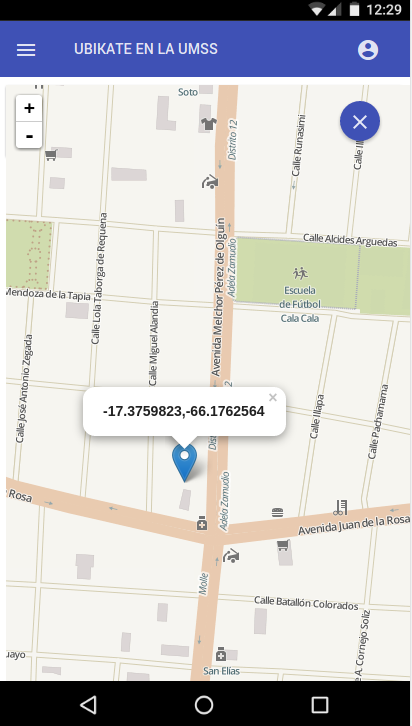
\includegraphics[width=0.5\textwidth]{iteration2/location_marker}
%     \caption*{Fuente: Elaboración propia.}
%   \end{center}
% \end{figure}



\subsubsection{Encontrar la ruta óptima entre el usuario y el lugar}

% \section{Ruta óptima dentro el Campus Universitario}
% \label{sec:generar_mapa_rutas}

Para solucionar este problema se necesita geolocalizar todas rutas que existen dentro del campus Universitario. \\

% Para responder al problema de encontrar una ruta óptima entre 2 puntos dentro del campus universitario, se necesita de un mapa que contenga todas las rutas que existen dentro del campus.\\

%
%
% \section{Campus Universitario}
% \label{sec:ruta_corta_umss}

% En primer lugar fue necesario obtener un grafo ponderado no-dirigido que representa un mapa de los caminos que existen dentro del campus Universitario.\\

Por lo que se procedió a caminar a través del campus Universitario con un \emph{GPS Garmin Nuvi 1300}, que es un dispositivo GPS básico pero puede guardar información geográfica,  se recorrió los principales caminos que existen e interconectan las distintas facultades y oficinas dentro del campus universitario. Una vez realizado este recorrido, se procedió a extraer la información del dispositivo GPS y exportarlo a un archivo \emph{shapefile}, para esta tarea se utilizó \emph{QGis}. \\
% con el cual se acabó editando las rutas recogidas por el GPS.\\

% \footnote{Un shapefile es un archivo de formato sencillo y no topológico que se utiliza para almacenar la ubicación geométrica y la información de atributos de las entidades geográficas.\cite{what_is_shapefile} }

Una vez exportado a un archivo \emph{shapefile} fue necesario editar la información recogida con el dispositivo GPS porque la ruta recogida por el dispositivo es una línea única, y para usarla como un \emph{mapa de rutas} o \emph{red topológica} necesaria para buscar una ruta óptima entre 2 nodos de la red, es necesario que la línea única sea dividida o separada en muchas líneas, este paso se lo realizó con \emph{QGis} con la opción de \emph{explode lines}. \\

% las cuales son las aristas y los extremos de las líneas serán los nodos o vértices del grafo,
% técnicamente esta línea única es representada como un \emph{POLYLINE} el cual consiste en una o más partes. Una parte es una secuencia conectada de dos o más puntos. Las partes pueden o no estar conectadas entre sí. Las partes pueden o no intersectarse entre sí, y para transformar este \emph{POLYLINE} necesitamos separar todas sus partes y convertirlas en objetos \emph{LINESTRING} únicos,  \cite{esri_shapefile} \\

Una vez realizado el paso anterior se obtiene un conjunto de \emph{LINESTRINGs} o líneas únicas, resultado que se puede apreciar en la figura \ref{fig:shapefile_umss_v1}. \\

% que son segmentos de líneas rectas interconectadas, el cual se usó como el  ``mapa de rutas''.



 % el grafo representa el mapa de caminos  pueda ser usado en una base de datos  “ruteable”, esto significa que el mapa de una sola línea hay que separarlo o dividirlo en muchas líneas.\\


\begin{figure}[H]
  \begin{center}
    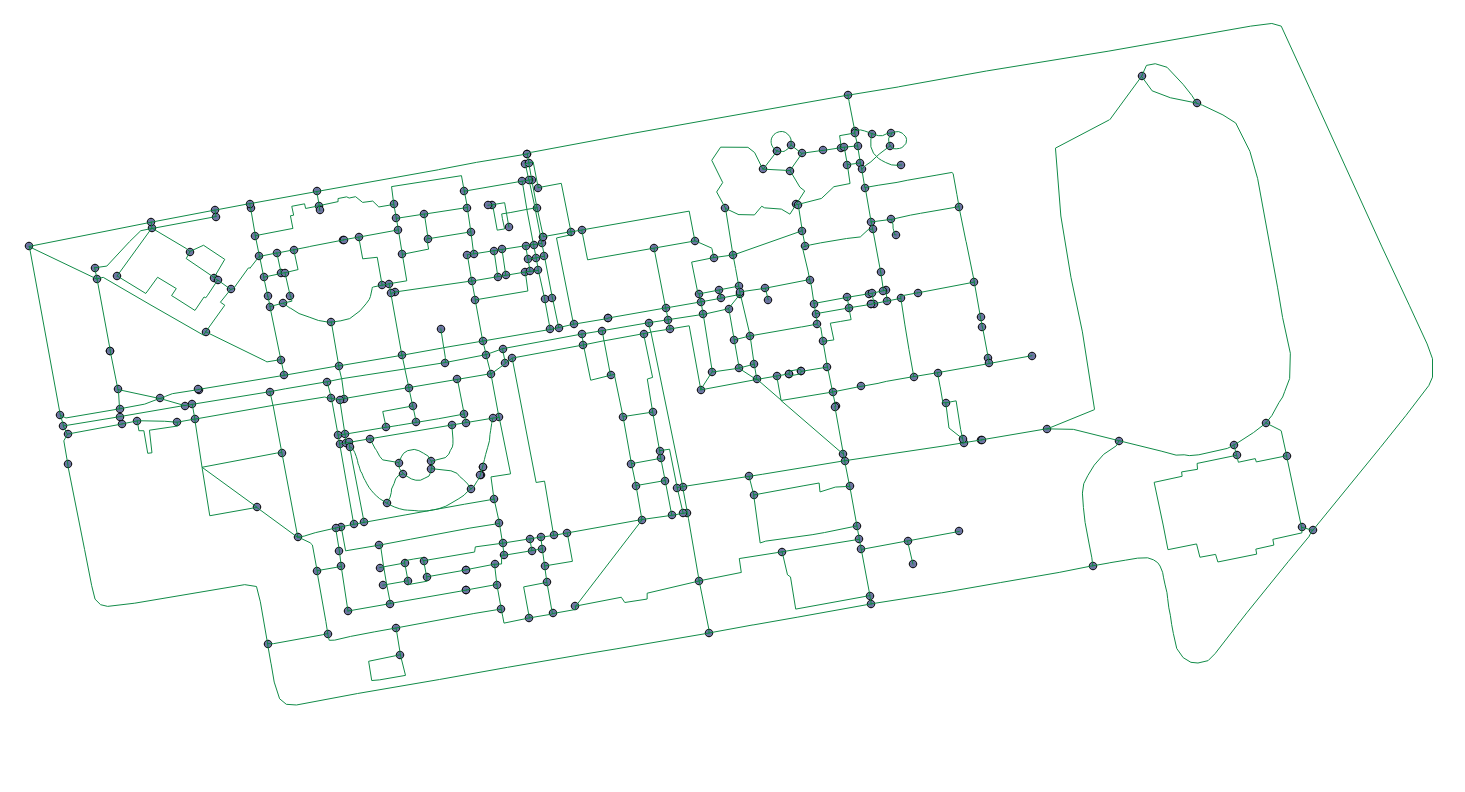
\includegraphics[width=1\textwidth]{shapefile_umss_v1}
    \caption{Mapa de rutas del campus Universitario.}
    \label{fig:shapefile_umss_v1}
    \caption*{Fuente: Elaboración propia}
  \end{center}
\end{figure}

% Este \emph{mapa de rutas} es un \emph{grafo no-dirigido} sobre el cual se aplicó el algoritmo de \emph{Dijkstra} encontrando la ruta más corta dentro del campus Universitario. \\

El mapa generado con las rutas cumple con las características de un \emph{grafo ponderado no-dirigido} en el que el costo o peso de las aristas es la distancia entre los nodos y los nodos son los puntos de intersección de las rutas. Por lo tanto se puede implementar el algoritmo de \emph{Dijkstra} para encontrar el camino mínimo. \\

Para la manipulación de las rutas georeferenciadas y la implementación del algoritmo de \emph{Dijkstra}, es necesario preparar la base de datos para tal tarea. Por lo cual se añadió la extensión \emph{pgRouting}, herramienta que ya tiene implementada el algoritmo de \emph{Dijkstra} y puede ayudar a encontrar la ruta óptima entre 2 nodos en una \emph{red topológica}.\\

% Para una mejor apreciación del grafo que consta de 1164 aristas y 1003 vértices, se lo puede ver en combinación o proyectada en un mapa de rutas del campus de la Universidad Mayor de San Simón ubicado entre las calles Oquendo, Sucre y  Belzu de la ciudad de Cochabamba - Bolivia, se puede referir a la siguiente figura \ref{fig:shapefile_umss_v2}.
%
% \begin{figure}[H]
%   \begin{center}
%     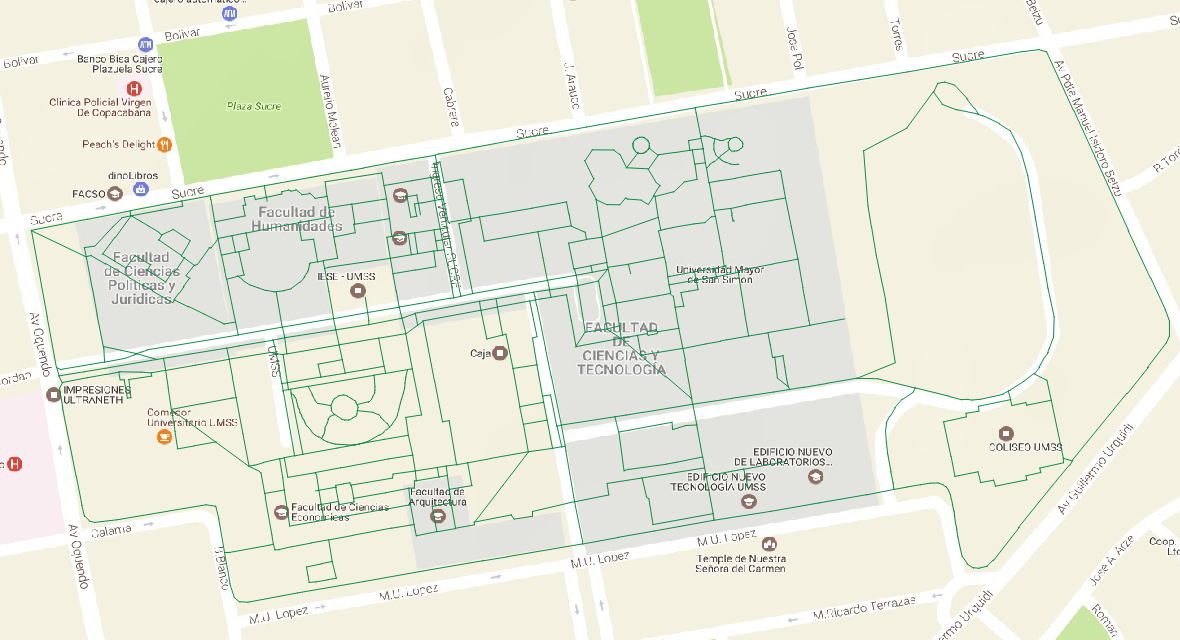
\includegraphics[width=1\textwidth]{shapefile_umss_v2}
%     \caption{Shapefile sobre el campus Universitario de la UMSS.}
%     \label{fig:shapefile_umss_v2}
%     \caption*{Fuente: Elaboración propia}
%   \end{center}
% \end{figure}


% \subsubsection{Las Rutas}
% \label{subs:Las Rutas}

% Después de generar el archivo shapefile, se procede a popular la base de datos del mismo modo que se hizo con la información de los lugares. Para las rutas se genera una tabla nombrada \emph{ways}.\\

Se creó la tabla \emph{ways} para que contenga las rutas georeferenciadas, para preparar esta tabla para que soporte las funciones instaladas por \emph{pgRouting} es necesario ejecutar un query propio de \emph{pgRouting}, se puede ver en el siguiente codigo, el cual tiene como objetivo analizar los datos geo-espaciales de la tabla y añadirle una \emph{topología}.\\

% Una vez poblada la base de datos se procede a cargar la misma con la información obtenida en RF011, para tal efecto es necesario primeramente crear una tabla que contendrá los LINESTRING contenidos en el shapefile, esta operación es similar a la realizada en la tarea - RF003 (\ref{sub:RF003}). Una vez que ya se tiene la tabla a la llamamos \emph{ways},

\begin{verbatim}
 select pgr_createTopology('ways', 0.00000001, 'geom', 'gid');
\end{verbatim}

Dentro lo que es la \emph{topología geoespacial} se denomina \emph{topología de red} a la representación de las relaciones entre segmentos en una red lineal o una colección de segmentos de línea. \cite{osgeo_journal_topology} \\

En un \emph{SIG} la topología ayuda a mejorar el análisis de datos geo-espaciales, para resolver el problema de la ruta corta \emph{pgRouting} genera una \emph{topología de red} usando los datos que existen en la tabla \emph{ways}, es necesario ejecutar una instrucción, la que se muestra a continuación y \emph{pgRouting} se encarga de llenar los datos que se pueden observar en la figura \ref{fig:postgres_ways}, las columnas \emph{source} y \emph{target} son populadas con el análisis topológico y en la figura \ref{fig:postgres_vertices}, se puede observar que la tabla \emph{ways\_vertices\_pgr} es creada enteramente en la ejecución de la instrucción.\\

\begin{figure}[H]
 \begin{center}
   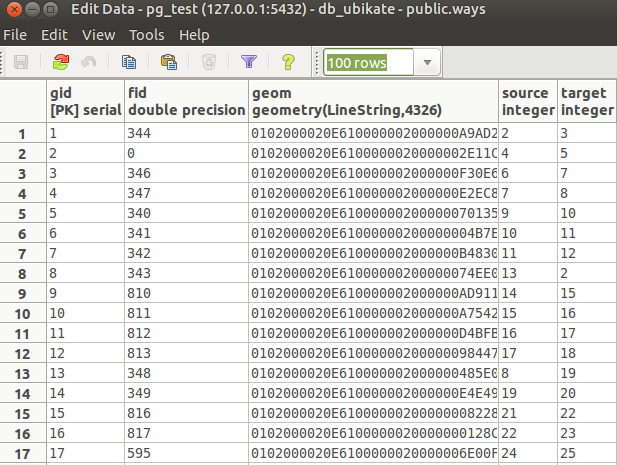
\includegraphics[width=0.8\textwidth]{iteration2/postgres_ways}
   \caption{Vista de la tabla \emph{ways}.}
   \label{fig:postgres_ways}
   \caption*{Fuente: Elaboración propia}
 \end{center}
\end{figure}

En la figura \ref{fig:postgres_ways} se puede apreciar que cada fila es una parte de la línea original obtenida por el dispositivo GPS y explosionada por QGIS, hay que notar que las columnas \emph{source} y \emph{target} hacen referencia a los nodos o vértices que la primera línea tiene en sus extremos, la primera línea o fila está identificada por la columna \emph{gid}.\\

En la siguiente figura \ref{fig:postgres_vertices} se observa la tabla \emph{ways\_vertices\_pgr} que contiene los vértices creados a partir del análisis de los datos en la tabla \emph{ways}.

\begin{figure}[H]
 \begin{center}
   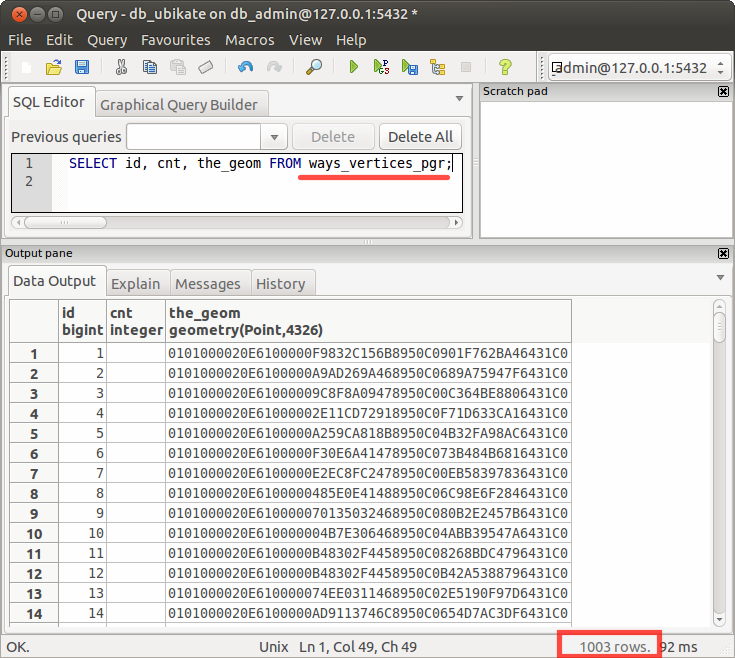
\includegraphics[width=0.8\textwidth]{iteration2/postgres_vertices}
   \caption{Vista de la tabla \emph{ways\_vertices\_pgr}.}
   \label{fig:postgres_vertices}
   \caption*{Fuente: Elaboración propia}
 \end{center}
\end{figure}

Para entender los datos generados hay leer la información de las 2 tablas, por ejemplo en la primera  fila (gid 1) de la tabla \emph{ways}, se observa que el contenido de la columna \emph{source} es igual a \textbf{2} y \emph{target} es igual a \textbf{3}, eso quiere decir que los vértices del LINESTRING de la fila 1 son los vértices con \textbf{id} 2 y 3 respectivamente de la tabla \emph{ways\_vertices\_pgr}.\\

% Todo el conjunto de vértices y líneas de estas tablas se podría representar con una Matriz de adyacencias, explicada en \ref{sub:representacion_de_un_grafo}, y usada en la resolución de la ruta mas corta, mas específicamente con el algoritmo de Dijkstra.\\

\emph{PgRouting} ya tiene implementado el algoritmo de \emph{Dijkstra}, pero solo puede ser utilizado cuando ya se le haya añadido una topología a la tabla con las rutas. En el siguiente codigo \ref{pgr_dijkstra}, se puede ver la consulta SQL utilizada para encontrar la ruta óptima entre 2 nodos de la red topológica.\\

\begin{center}
 \begin{lstlisting}[label=pgr_dijkstra,caption=Algoritmo de Dijkstra implementado en \emph{pRouting}]

   SELECT seq, id1 AS node, id2 AS edge, cost
   FROM pgr_dijkstra(SELECT gid AS id,
                             source::integer,
                             target::integer,
                             st_length(geom) AS cost
                      FROM public.ways, targetId, sourceId, false, false);

 \end{lstlisting}
\end{center}


% La anterior consulta SQL es una llamada al método \emph{pgr\_dijkstra} implementado en \emph{pgRouting} el cual solo puede ser utilizado una vez que la base de datos está preparada para tal efecto, es decir necesitamos que la tabla de rutas \emph{ways} tenga la topología de red y también

Los nodos de destino y origen, \emph{targetId} y \emph{sourceId} respectivamente, son datos obtenidos por una combinación de acciones ya que los nodos son propios del mapa de rutas ubicados en la tabla \emph{ways} y el punto destino que se están utilizando es en realidad un \emph{lugar} del campus Universitario ubicado en la tabla \emph{places} y el punto origen es la posición actual del usuario. Por lo que para obtener los nodos utilizados en la consulta SQL, es necesario encontrar los nodos ``más'' cercanos a estos puntos y gracias \emph{PostGIS} encontrar encontrar el nodo más cercano, se necesita ejecutar la siguiente consulta SQL, donde \emph{lon} y \emph{lat} son la longitud y latitud de los puntos origen o destino. \\

\begin{verbatim}
   SELECT id
   FROM ways_vertices_pgr
   ORDER BY the_geom <-> ST_GeometryFromText('POINT(lon lat)', 3857)
   LIMIT 1
\end{verbatim}

Una vez ejecutado el método \emph{pgr\_dijkstra} se obtiene un conjunto de líneas, que son un conjunto de latitudes y longitudes que representa la ruta más corta entre el punto origen y el punto destino, esta informacion realmente no dice nada a la persona que lo lee por lo tanto requiere ser procesada para poder ser consumida desde el navegador, este proceso es llevada a cabo en el servidor y entregada al cliente en formato GeoJSON.\\







Entonces se obtiene
% poder mostrar la ruta óptima es necesario obtener
de la base de datos un conjunto de datos en formato de latitud y longitud que conforman líneas, las cuales representan la ruta más corta, pero al final es solo un montón de números, sin mucho significado para el usuario, toda esta información es difícil de procesar y el usuario necesita información que sea fácil de entender y no existe mejor herramienta disponible para esta tarea que mostrar la \emph{ruta} de forma visual, esto quiere decir que se necesita mostrar la ruta sobre un \emph{mapa}, ya que en la aplicación se implementó \emph{ember-leaflet} para desplegar el mapa y mostrar un lugar, también se puede  mostrar más ruta más corta mediante una línea, a la que también se puede personalizar (la línea se muestra de color rojo).\\

A continuación se puede apreciar el \emph{request} que el frontend hace al API y  el objeto GeoJSON que es recibido, este objeto contiene la información geoespacial necesaria para ``dibujar'' la línea roja entre 2 puntos georeferenciados, uno de los puntos es donde se encuentra el usuario (\emph{sourceData}) y el otro punto es el lugar (\emph{targetData}).
% A continuación se puede apreciar el request al API

% uno de los cuales es el lugar al que se quiere llegar y el otro es la ubicación actual del usuario. \\

% ENV.APP.API_HOST + '/api/v1/ways/route/' + sourceData.id + '/' + targetData.id;


\begin{center}
  \begin{lstlisting}[label=call_ways,caption=Llamada al \emph{endpoint} que retorna la ruta óptima.]

    GET /api/v1/ways/route/930/77 200 276.217 ms - 3911

    $ curl http://localhost:3000/api/v1/ways/route/930/77 | python -m json.tool
  {
      "features": [
          {
              "geometry": {
                  "coordinates": [
                      [
                          -66.1467397848201,
                          -17.3935321732846
                      ],
                      [
                          -66.1467190789842,
                          -17.3935294725234
                      ]
                  ],
                  "type": "LineString"
              },
              "type": "Feature"
          },
          .
          .
          .
     ]
 }

  \end{lstlisting}
\end{center}

\begin{verbatim}

\end{verbatim}
% /api/v1/ways/route/

Una vez que se tiene los datos, es necesario representarlo en el mapa y para tal efecto se seguirá utilizando \emph{ember-leaflet} y que con el tag \emph{geojson-layer}, ver el siguiente codigo, se puede observar en el mapa una línea roja que representa la ruta más corta entre el punto donde se encuentra el usuario y el punto del \emph{lugar}. Tal como se puede apreciar en la figura \ref{fig:short_way_place}.
% Este objeto es representado en el mapa usando ember-leaflet con la siguiente instrucción,
%
\begin{verbatim}
 {{#geojson-layer geoJSON=currentGeoJSON color='red' }}
\end{verbatim}

% Se puede

\begin{figure}[H]
 \begin{center}
   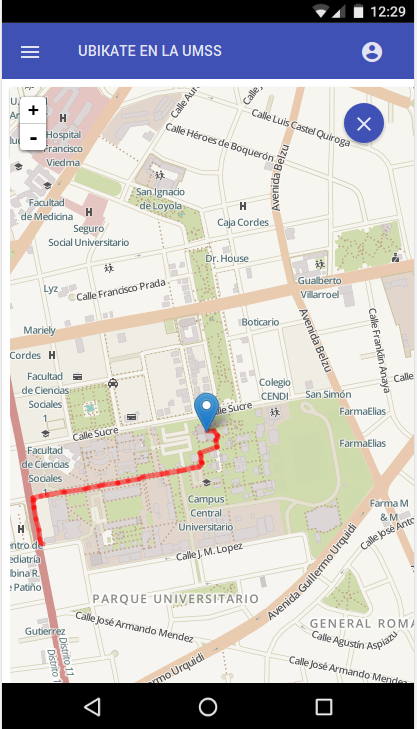
\includegraphics[width=0.3\textwidth]{iteration2/short_way_place}
   \caption{Ruta más corta dibujada con una línea roja.}
   \label{fig:short_way_place}
   \caption*{Fuente: Elaboración propia.}
 \end{center}
\end{figure}



% Para dibujar líneas rectas sobre un mapa hay que tomar en consideración que la tierra no es plana y las líneas que en un mapa parecen líneas rectas, realmente no son rectas, ya que el planeta Tierra es un \emph{esferoide oblato}\footnote{Un \emph{esferoide oblato} (o elipsoide oblato) es un elipsoide de revolución obtenido por rotación de una elipse alrededor de su eje más corto.} por lo que las líneas en apariencia rectas tienen la curvatura natural del planeta Tierra. En distancias largas esto tiene un gran impacto al manejar o utilizar mapas proyectados, pero también es cierto que para una área pequeña como es el campus de la Universidad de San Simón este problema no tiene un gran impacto pero no está demás en tomar en cuenta esta característica en el análisis de datos geoespaciales, como se explicó en el capitulo \ref{cha:geolocalizacion}, para el presente proyecto se usará el proyección \emph{SRID 3857}.\\
